In order to build a \textbf{Zero Trust AuthZ protocol}, it is necessary to build around \textbf{trust}, 
and design an engine capable of elaborating this trust dynamically, filling the gap beyond simple token delivery.  
This work has started under the name \textbf{ZTAuth* (Zero Trust Auth*)}.  
Such a system must rely on \textbf{autonomous components}, able to operate even in case of disconnections.  

\vspace{0.5em}  
A Zero Trust architecture must include a \textbf{Policy Decision Point (PDP)} built around Zero Trust principles.  
The first point to understand is that when a PDP is asked to take a decision, there are always \textbf{two identities} involved:
\begin{itemize}
    \item the identity of the \textbf{workload} requesting the decision (it cannot be manual, otherwise it would not scale);
    \item the identity of the \textbf{subject} (human or non-human) that is the target of the evaluation.
\end{itemize}
These identities may be expressed via \textbf{tokens}, \textbf{SPIFFE}, \textbf{ZCAP-LD,}, or any other valid identity proof.  

\vspace{0.5em}  
In this way, a \textbf{Trust Chain} can be built as the composition of multiple \textbf{Trust Inputs}, 
possibly with parallel branches. These inputs must connect with autonomous components 
and be usable across multiple transport layers.

The PDP receives as input an \textbf{authorization context}, which includes:
\begin{itemize}
    \item the subject identity proof and related attributes (possibly from a \textbf{Policy Information Point (PIP)}),
    \item the workload identity proof,
    \item information about the action requested.
\end{itemize}
Each of these is a \textbf{trust input}, which may be a token, a contextual signal, or other forms of trust such as \textbf{UCAN} or \textbf{ZCAP-LD}, depending on the use case and flow.  

\vspace{0.5em}  
To evaluate a request, the PDP must already have access to:
\begin{itemize}
    \item a synchronized set of \textbf{policies},
    \item additional \textbf{trust statements} (e.g., UCAN, ZCAP-LD, or others),
    \item a mechanism for decision \textbf{logging and auditing}.
\end{itemize}

\vspace{0.5em}  
During evaluation, the PDP creates an \textbf{authorization context} for the workload, 
verifying whether it can act on behalf of the subject.  
If conditions are satisfied, the system may perform a \textbf{Trust Elevation}, 
allowing the workload to inherit subject permissions.  
System owners must also be able to define under which conditions this is allowed, 
possibly grouping workloads into \textbf{Trust Levels}, which require synchronization and governance.  

\begin{boxF}
Example: John has a valid OAuth token to print a document, 
but policy restricts classified documents to printers in a secure segment with verified workload identity.  
Even with a valid token, printing must be blocked if the printer is not trusted at that moment.
\end{boxF}

Finally, the model must define how \textbf{Trust Delegation} works, 
ensuring safe delegation of rights across entities.

\begin{figure}[htbp]
    \centering
    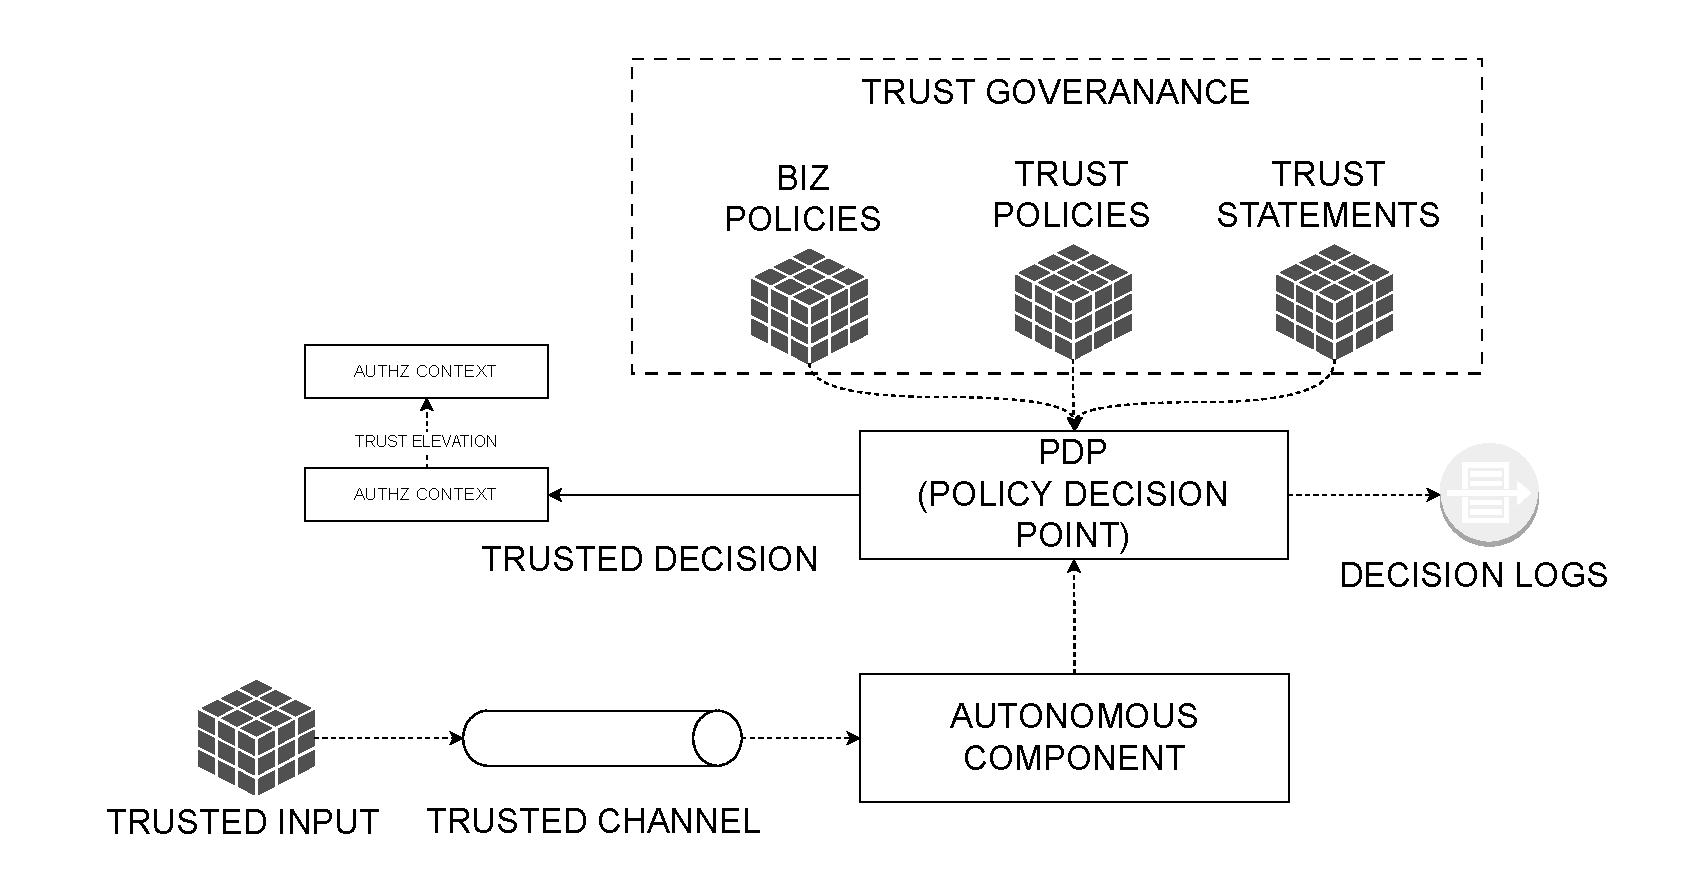
\includegraphics[width=0.5\textwidth]{authz/authzprotocol.pdf}
    \caption{AuthZ Protocol}
    \label{fig:authzprotocol}
\end{figure}

\vspace{0.5em}  
To enable such a protocol ref{fig:authzprotoco} , it is necessary to define and standardize:
\begin{itemize}
    \item \textbf{Trust Inputs},
    \item \textbf{Trust Decisions},
    \item \textbf{Trust Elevation},
    \item \textbf{Trust Levels},
    \item \textbf{Trust Delegation}.
\end{itemize}
